\chapter{Modélisation des données et Évaluation}
\epigraph{Economists and agronomists are locked in debate about likely
future yields. Since the method of the economists is to predict
future outcomes from past performance, economists expect
success to continue. And since for the scientists future success
depends on discoveries they will have to make and do not now
know how to make, the scientists are doubtful. At its core, this is
a disagreement about the pace of technical change.}{Robert
Socolow}
\cleardoublepage

	\section{Analyse causale}
		\shorthandoff{!}
		\lstset{language=R}
		\shorthandon{!}
	\subsection{Introduction à la régression en composantes principales}
	Les méthodes de régression multivariée comme la RCP\footnote{Régression en composantes principales} jouissent d'une large popularité dans divers domaines d'études, y compris les sciences naturelles. La raison principale de ce succès étant qu'elle ont été conçues dans l'optique de faire face à des situations où on dispose de plusieurs variables exogènes, généralement hautement corrélées, et relativement peu d'échantillons. Une situation qui est justement notre problématique. Ainsi une forme de réduction de dimensions dans l'espace des exogènes peut grandement simplifier le problème de régression.L'analyse en composantes principales est une technique de réduction de dimensions où une combinaison linéaire de \textit{p} variables indépendantes/orthogonales des paramètres intrants $X_1,X_2,...X_p$ sont créées de façon à ce que la première combinaison linéaire $Z_{1}$ (composante principale) capture autant de la variance totale des données d'origine. La $2^{de}$ $Z_{2}$ capture autant que possible du reste de la variance sous la réserve que celle-ci soit orthogonale(i.e. non corrélée) à la première. En général toutes les variables intrantes sont standardisées de façon à posséder une moyenne nulle et une variance unitaire que l'on notera $X_{j}^{*}$. Ainsi la variance totale des \textit{p} intrants standardisés est donnée par :
	\begin{equation*}
	\sum_{j=1}^{p} V(X_{j}^{*}) = p = \sum_{j=1}^{p}V(Z_{j})
	\end{equation*}
	avec $\forall i \in [1,p]$:
	\begin{equation*}
	Z_i = \sum_{j=1}^{p} a_{ij} X_{j}^{*} 
	\end{equation*}
	et $\forall i \neq j$
	\begin{equation*}
		Cov(Z_i,Z_j) = Corr(Z_i,Z_j) = 0
	\end{equation*}
	Les composantes principales sont déterminées par l'analyse spectrale (i.e la recherche des valeurs propres et vecteurs propres) de la matrice des corrélations des variables intrantes. La variance de la $j^{eme}$ composante principale $Z_{j}$ est $\lambda_{j}$ la $j^{eme}$ valeur propre la plus grande. Les coefficients $a_{ij}$ de la combinaison linéaire sont les vecteurs propres correspondant.\par
	Idéalement les \textit{k} premières composantes principales comprendront une part consistante de la variance totale des données. Nous pouvons par la suite utiliser ces \textit{k} principales composantes $Z_1,Z_2,...X_k$ comme variables exogènes dans le modèle de régression linéaire multiple:
		\begin{equation*}
		Y=\beta_0 + \sum_{\j=1}^{k} \beta_jZ_j + \epsilon 
		\end{equation*}
	Dans ce qui suit nous mettons en œuvre une RCP sur nos données élaguées obtenus après le traitement du chapitre précédent. Le script en langage \textbf{R}, avec lequel la RCP est automatisée, est disponible dans le dossier \textit{Source} de notre dépôt PFE \textbf{GitHub}\cite{this}.
	\subsection{Mise en œuvre de la régression en composantes principales}
	\subsubsection{Corrélations croisées des variables exogènes}
	Nous commençons d'abord par charger les données quantitatives des pays. Il s'agit de l'élagage des données externes présentées à la section \ref{exoList}. Ces données représentent, de la totalité des 39 variables initiales, les 12 variables retenues en sortie de la procédure introduite par les forets aléatoires en section \ref{faout} avant de créer deux matrices:\begin{itemize}
	\item DF.actifs = Cette matrice accueillera les 12 variables retenues dans la figure \ref{fig:laggedvars}.
	\item DF.illus = Cette matrice-vecteur accueillera notre variable de sortie qui est la \textbf{Consommation de kilogrammes de fertilisants phosphatés par hectare de terre arable} 
	\end{itemize}
	Commençons d'abord à chercher les variables relativement colinéaires. Nous donnons dans la figure \ref{fig:scatter} les diagrammes de dispersions deux-à-deux croisés entre les 12 variables de notre modélisation. Nous joignons à ceux-ci des courbes splines facilitant la détection de structure ainsi qu'en gras les valeurs des coefficients de corrélations les plus importants.
			\begin{figure}[h]
				    		\centering
				    		\fbox{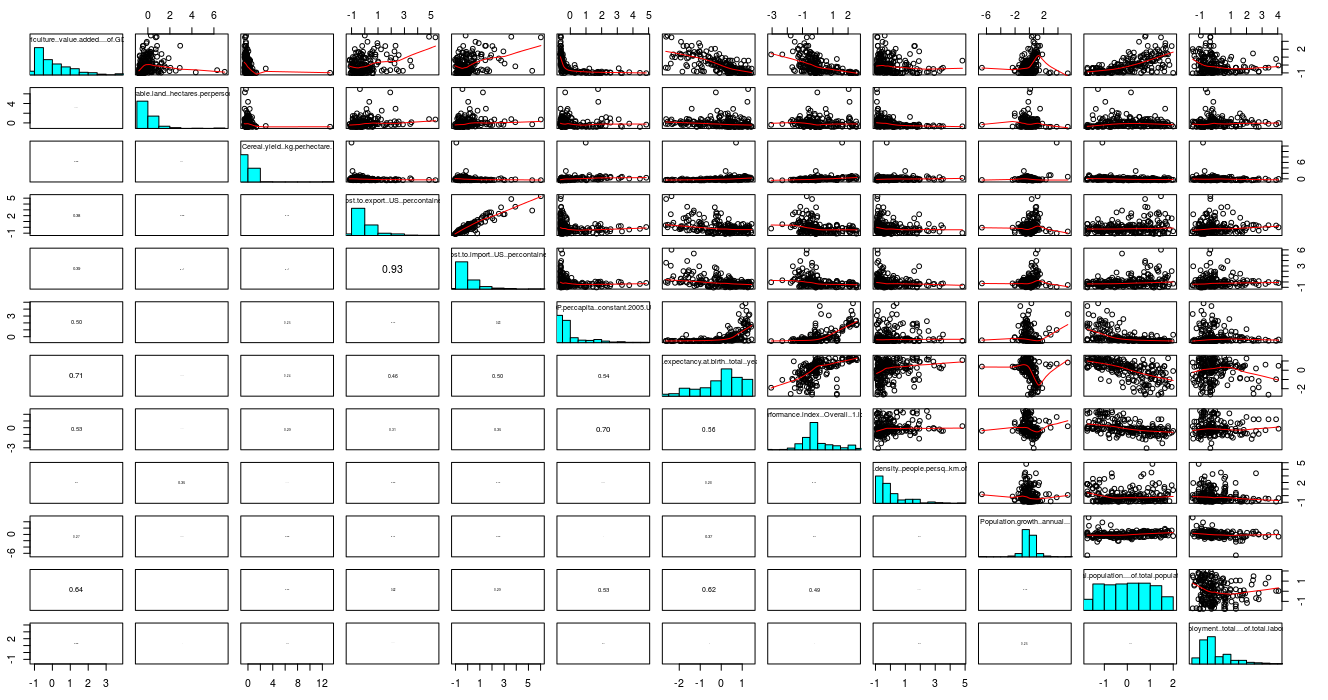
\includegraphics[width=\linewidth]{ch4-images/scatter}}
				    		\caption{Diagrammes des dispersions croisées, courbes splines et corrélations des variables exogènes}
				    		\label{fig:scatter}
			\end{figure}
	Plusieurs couples de valeurs présentent des corrélations sensiblement élevées en valeurs absolues:
	\begin{itemize}
	\item \{Coût d'import conteneur Vs Coût d'export conteneur\}
	\item \{\%(Agriculture) du PIB Vs Espérance de vie\}
	\item \{PIB par habitant Vs Indice de performance logistique\}
	\item \{\%(Agriculture) du PIB Vs \%(Population rurale) de la population totale\}
	\item \{Indice de performance logistique Vs Espérance de vie\}
	\item Certaines de ces variables entre elles par transition des couple ci-dessus.
	\end{itemize}
	Une autre façon d'examiner la structure des corrélations est la création de carte coloriée dressant les corrélations deux à deux entre les variables numériques. Ceci sont \textit{clusturisés} et ordonnés aux seins de groupes de variables corrélées. Sur la figure \ref{fig:heatmap} nous pouvons distinguer 4 à 5 groupes de variables exogènes corrélées. Ainsi une ACP devrait produire 4 à 5 composante principales intégrant la majorité de l'information contenue dans les données.
				\begin{figure}[h]
					    		\centering
					    		\fbox{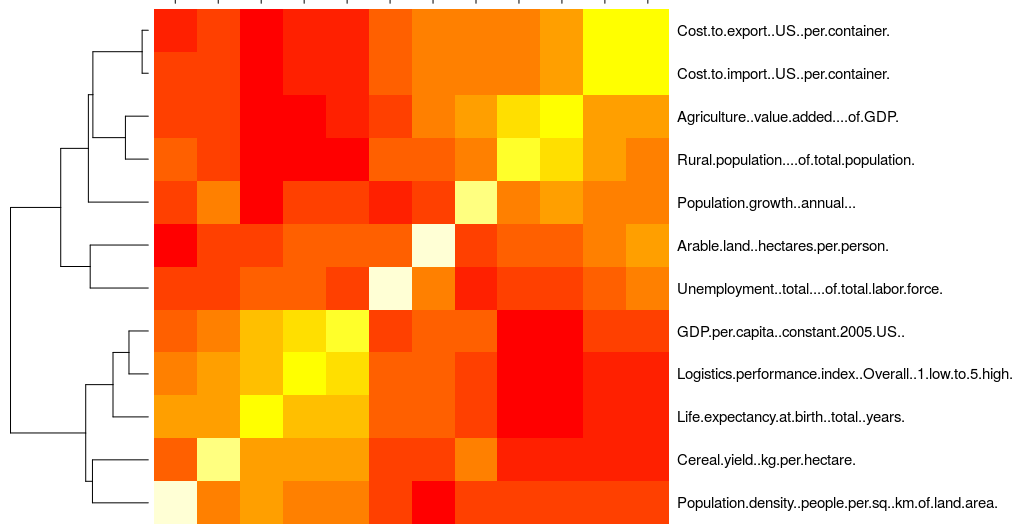
\includegraphics[width=\linewidth]{ch4-images/heatmap}}
					    		\caption{Carte coloriée des regroupement des variables corrélées}
					    		\label{fig:heatmap}
				\end{figure}
	\subsubsection{Calcul des composantes principales des données élaguées}
	Nous commençons par effectuer une décomposition spectrale de la matrice de corrélation. La figure \ref{fig:valpropres} ci-dessous liste les valeurs propres résultant de cette décomposition.
				\begin{figure}[h]
					    		\centering
					    		\fbox{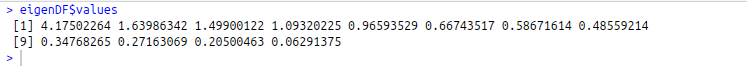
\includegraphics[]{ch4-images/valeurs_propres}}
					    		\caption{Valeurs propres de la décomposition spectrale de la matrice de corrélation}
					    		\label{valpropres}
				\end{figure}
	La figure \ref{fig:inert} suivante montre que 70\% et 78\% de l'inertie de l'ensemble des données est exp
	\section{Analyse en séries chronologiques et projections}
	\begin{Huge}{ En cours de construction}
		\end{Huge}